\documentclass[11pt, a4paper, notitlepage]{report}
\newcounter{objectivesCounter}
\usepackage[utf8]{inputenc} % Ensures we can use UTF8.
\usepackage[round,colon]{natbib}
\bibliographystyle{hull}
\usepackage{amsmath}
\usepackage{graphicx}
\graphicspath{ {./images} }
\usepackage{hyperref} % Must come last; allows for links.
\hypersetup{
    hidelinks
}

\title{Smart Kart}
\date{April 2022}
\author{George Jacob Anthony Kokinis}
\begin{document}
\begin{center}
	{\Huge Smart Kart}
	
	\bigskip
	{\Large Final Report}
	
	\bigskip
	Submitted for the BSc in
	
	\bigskip
	{\LARGE Computer Science}
	
	\bigskip
	April 2022
	
	\bigskip
	by 
	
	\bigskip
	{\LARGE George Jacob Anthony Kokinis}
    
    \bigskip
    Word Count: ?? %exclude acknowledgements, abstract, table of contents, references and appendices) of your document.
\end{center}
\newpage
\section{Abstract}
Average speed check zones (ASC zones), typically enforced using SPECS\footnote{SPECS \citep{specsjenop}} in the UK, are being increasingly deployed throughout the UK, doubling between 2013 and 2016 \citep{BBCSpeedCameraDoubled}. While useful for enforcing speed limits and increasing safety, with \citet{owenAllsop} finding that fatal and serious collisions dropped by 36.4\% at ASC zones installed purposely to reduce collisions, ASC Zones can lead to distracted driving, as the driver has to monitor their speed, which means looking away from the road to their speedometer for brief periods of time.

This project seeks to create a software application for a smartphone, that detects when a vehicle the phone is in enters an ASC zone, starts tracking the vehicle's speed, and gives the driver an audible alert if their average speed is at risk of breaking the speed limit, thereby reducing dependence on the driver to check their speedometer.

\section{Acknowledgements}
I would like to acknowledge the invaluable contributions of Eur Ing Brian Tompsett and Lydia Bryan-Smith (both, at the time of writing, of Hull University) with regards to \LaTeX\ typesetting; without their guidance I would be stuck with regards to some of its peculiarities.

My Grandfather, Alec Kokinis, provided instrumental help in proof-reading this document. Thank you.

\tableofcontents

\chapter{Introduction}
\section{Context}\label{sec:Context}
Average speed check zones are an alternative to traditional fixed point speed cameras. Fixed point cameras take two photos a given time-delta apart and measure the car's distance using road markings, to calculate the speed: $ speed = distance \div time $. This is good for enforcing speed in that one position, but provides no enforcement for the road before or after the camera. In contrast, ASC zones effectively use the same methodology but across a longer distance (such as half a mile or 1.5 miles between cameras, and a series of cameras across tens of miles); hence effectively enforcing the speed limit across much larger areas of road.

Currently, there are various products for monitoring a driver's speed and for indicating speed cameras; the main smartphone applications in this space are Google Maps \citep{googleMaps} and Waze \citep{waze}; while Apple Maps \citep{appleMaps} will inform the user of fixed speed cameras\footnote{In the UK, these were originally "Gatso" cameras, later followed by Truvelo and Truvelo d-cam \citep{dcam}}, it does not inform of ASC zones.

However, Google Maps does not register ASCs as actual "zones", but instead as a fixed speed camera at the start of the zone. Waze displays progression through an ASC, but does not calculate average speed. TomTom GO Navigation \citep{tomtomGo} does track average speed in an ASC zone, but operates on a paid subscription model, so is not available to everyone. Hence, there is space in the market for a free solution to monitoring speed in ASC zones.
\section{The Problem}
While conscientious drivers should be aware of their speed anyway, it is likely that many check their speed more often and with more discretion whilst within an ASC zone. This means they may be focused on their speedometer when something important is passed, such as a direction sign, a signal from another road user, or an overhead gantry message - such as the "Red X" on Smart Motorways\footnote{Smart Motorways \citep{SmartMotorways}}, or a speed limit change.
\section{A Solution}
By creating a smartphone application that warns a user if they are about to exceed the speed limit, the load on the driver can be reduced, allowing them to have more awareness of the road. By making this application free to use (whether free or supported by advertisements), this increases availability, potentially increasing the impact of this project.
\section{Report Structure}
The rest of this report is structured into the following chapters:
\begin{itemize}
	\item Background: Describing and laying out technologies and concepts that may be used in the development of the application or are useful for understanding other technologies.
	\item Aims and Objectives: Specification in detail about what features the application should have and how this will be tested or measured.
	\item Design: A description of the initial design, visual and technical, for the application, and design(s) for surveys to gain feedback on the UI of the application.
	\item Technical Development: Discussion around the development of the application. Note that the actual development log will be listed in Appendix \ref{app:GitLog}.
    \item Evaluation: Discussion and Evaluation of how closely the application meets the Aims and Objectives in the aforementioned chapter.
\end{itemize}
After which there will be Appendices and the Bibliography. % Remove this?
\chapter{Background}
The development of this project requires understanding and examination of various topics across various fields; including Kinematics, Programming, Law, and UX. Hence this chapter discusses and describes relevant topics.
\section{Speed Cameras}
\subsection{Fixed-Point Cameras}
In the United Kingdom, traditional fixed-point speed cameras were of a "Gatso" type, later replaced by "Truvelo", and later Truvelo D-Cam. They are installed either by the Local Authority, the local Police Force, or the relevant highways agency\footnote{\textit{National Highways} in England, \textit{Transport Scotland} in Scotland, \textit{Traffic Wales} in Wales, and \textit{DfI Roads} in Northern Ireland.}; with all three often forming "Road Safety Partnerships" for given areas, that can then receive grants from the central government \citep{RSPGrantDetails} to use for, among other things, the installation of speed cameras. The decision of where to install a speed camera is made on a few factors; with \citet{SpeedCameraInstalltion} claiming that at the proposed location, greater than 20\% of drivers must exceed the speed limit, and that there must be a history of serious accidents.

At first glance, fixed-point cameras appear to work on a rather simple principle. As described in the \nameref{sec:Context}, the simplest view of how to obtain the speed of a vehicle is $ speed = \frac{distance}{time} $. Hence the camera can take two measurements a known time apart, work out the distance the vehicle travels between those measurements, and calculate the speed. 
Fixed-point cameras use K and Ku-band Radar signals to determine the speed of the vehicle; K-band meaning that the frequency used is between 18 and 27 GHz \citep{IEEERadar}; and Radar, an acronym for Radio Detection and Ranging \citep{RadarNaming}, referring to the usage of a transmitter, receiver, and processing of K-Band or adjacent frequencies (in the Radio or Microwave ranges) to determine properties of an object. The time of flight is the total time between transmitting a signal and receiving the reflection; and this can be used to determine the distance. The speed of light is known\footnote{299 792 458 metres per second in a vacuum, known as \textit{c}, and slower in air: which can be calculated with $ speed = c \div n $ \citep{HechtOptics}; where n is the refractive index of the medium. \citet{refIndxAir} gives 1.0003 as the approximate refractive index of light in air; approximate as it can be affected by factors such as moisture content.}, and so the distance can be calculated using a rearrangement of the previous formula: $ distance = speed  \cdot time $. Hence, overall, the speed of a vehicle travelling towards/away from the camera can be calculated by:
\begin{equation}
	c' = \frac{c}{1.003}
\end{equation}
\begin{equation}
	first~measurement = c' \cdot time~of~flight
\end{equation}
\begin{equation}
	second~measurement = c' \cdot time~of~flight
\end{equation}
\begin{equation}
	speed = \frac{\left|second~measurement~-~first~measurement\right|}{time~between~measurements}
\end{equation}

However, this requires storage and memory of two time of flight measurements, and two distance measurements. Instead, an inherent property of waves can be used to determine the speed. The Doppler effect, first described by \citet{dopplerGerman} but better described for Radar applications by \citet{dopplerWolff}, is the property of waves that, as an emitter moves away or towards a stationary receiver (or vice versa), there is an apparent change in the frequency. The frequency is higher if the motion is towards the stationary point, as the receiver will receive a greater number of waves per second; and lower frequency if motion is away from the stationary point as it receives less waves per second. Due to this, the "doppler shift" - the difference between real and effective frequency, $ \Delta f $ - can be calculated as follows:
\begin{equation}
	\Delta v = -(v_{receiver} - v_{source})
\end{equation}
\begin{equation}
	\Delta f = \frac{\Delta v}{c'} \cdot f_{emitted}
\end{equation}
In the case of the speed camera, we can control $ f_{emitted} $, and we must take into account the fact that doppler shift will occur twice. Hence, the velocity $ v $ of a car can be calculated as such:
\begin{equation}\label{eq:DopplerSpeed}
	v = \frac{\Delta f}{f_{emitted}} \cdot \frac{c'}{2}
\end{equation}

If the vehicle's velocity calculated by equation \ref{eq:DopplerSpeed} exceeds the road's speed limit, the camera takes two photos in quick succession. In the original Gatso cameras these photos were on photographic film, which would be collected and processed by the local police force on a regular basis. Retrofitted Gatso and the newer Truvelo \& DCam systems upload their photographs and Radar Measurements to a system with the local Police Force; these systems are believed to be connected with the Police National Computer (PNC) \citep{PNC}. These photos contain the registration plate of the vehicle\footnote{Gatso cameras must take a photo of the rear of the vehicle due to the use of a bright flash, so will always obtain the registration plate; but do not photograph the driver and so the identity of the offender can be disputed. Truvelo \& DCam may take photos of the front, thereby identifying the offender, but some vehicles lack front plates.}, and markings on the road. These markings are graduated and are used to determine the distance the vehicle travels between the photos, and hence a speed can be determined; this \textit{secondary measurement} is used by prosecution teams to confirm an offence was made, but is not absolutely needed for a prosecution.

\subsection{Average Speed Cameras}
It may be wise to think, since average speed cameras were introduced after fixed-point cameras, that they would be significantly more advanced. In some ways they are, but in other ways they are much simpler.

\citet{ANPRNPCC} tells us that ANPR, Automatic Number Plate Recognition, refers to the reading of vehicle number-plates using OCR\footnote{Optical Character Recognition \citep{OCR}.}, storing information about those number-plates (such as the location and time of the scan), and querying a central system (such as the PNC) for details about the vehicle and its registered keeper. Number plates in the UK and generally in the EU are retroreflective; meaning that light is reflected back in direction it came from. Hence, most ANPR systems, including those used by Average Speed Cameras, take photos and use a flash in the infrared range to take a clearer image of a number plate.

Average Speed Cameras are deployed as systems consisting of multiple ANPR-equipped cameras, at known intervals, along a road or roads. These cameras can be permanently installed along roads, or temporarily installed at the site of roadworks. Installations come in various forms; they are installed on their own poles, on existing street furniture (EG lampposts), and on overhead gantries. The system has knowledge of the road distance (as opposed to direct distance, colloquially "as the crow flies") between cameras, and uses this knowledge combined with timestamped photographs of vehicles passing the cameras (with ANPR being used to match number-plates to timestamps) to calculate an average speed. This average takes into account factors such as changing lanes, and using junctions in an attempt to defeat the system.

A given system must have at least two cameras (so there are two measurements to calculate speed from), but there is no legal or algorithmic upper bound on the number of cameras in, or the length of, a single system \citep{cbASC}. Any upper bound is likely to be budgetary, technological, or jurisdictional; that is, the authority responsible for the system cannot afford the number of cameras, the computers to store and process data from the cameras, or legally cannot deploy cameras past a county or city boundary.

Put simply, average speed cameras go back to using the simple equation of $ speed = \frac{distance}{time} $. By applying this over a larger distance of road, rather than a small section, it encourages drivers to stay at or below the speed limit, and to drive in a smoother manner.

\subsection{Summary}
With regards to the application this project produces, from the previous knowledge, the following factors should be noted:
\begin{itemize}
    \item Fixed-point cameras are not relevant to average speed cameras in terms of applied technology, and therefore aren't relevant to the application. At most, there may be scope to provide notice of fixed cameras within the app.
    \item There is no public knowledge of pairing between any two cameras in a system; they may be paired sequentially or randomly.
    \item Hence, if a dataset has specific locations of cameras within a system, it is reasonable that average speed should be calculated between sequential cameras - IE between the current position and the previous camera, then reset at the next camera.
    \item If the dataset does not have specific locations, and only the start and end, then the average speed should be calculated between the start and end.
\end{itemize}

\section{Predicting Speed}
The change in speed over time, acceleration, is
\begin{equation}\label{eq:Accel}
    a = \frac{v - u}{t}
\end{equation}
This allows for finding change of speed in the past; but the application must effectively forecast whether a user's vehicle is going to exceed the speed limit. \citet{accelerationForecasting} provide and validate a model to predict maximum acceleration for trucks (LGVs). However it does not suggest whether their model works for smaller vehicles, and the model requires input parameters of tractive effort calculated from transmission efficiency, current speed, engine power, etcetera; it's a very comprehensive model, but an average driver may not want to go and find these details for their vehicle just to track average speed. Hence this model is unsuitable for the application; however the methodology may be useful to analyse.

Instead of a complex model, the application can just use past acceleration to predict future speed. This is naive model, but by using appropriate development techniques such as separation of concerns, this model can be changed for a more accurate one in the future. The basis, then, is a simple rearrangement of \ref{eq:Accel}:
\begin{equation}
    v = u + a \cdot t
\end{equation}
The main tuning parameter of this model for forecasting is t, time; whether this is user configurable (a setting saying "Notify me t seconds before exceeding the limit") or "hardcoded" is a consideration to be made. As well, this needs to be used with some hysteresis; it will be exceedingly annoying to the user if the application constantly alternates the alerting state.

\section{Programming and Development}
There are various options for platforms on which this application could be developed. This section discusses options, and ultimately decides as to which platform should be used.

\subsection{Cross-platform frameworks}
One contemporary paradigm is the use of cross-platform frameworks; where a developer writes their code using provided libraries, and the framework handles the "mapping" between calls into the libraries and the various host features. These frameworks can range from intrinsic to the language - in the case of Java and the openJDK \citep{openJdk}, where a JVM is almost completely necessary for running the program and so is provided by the Java developers - to external frameworks developed by entities separate to those who develop the language.

\paragraph{Flutter}
Flutter \citep{FlutterWebsite} is a cross-platform framework provided by Google (but is open source, so can be modified by the general public) that allows developers to build "multi-platform applications from a single codebase". It uses and itself is written in Dart, Google's "client optimized language for fast apps on any platform" \citep{dartWebsite}. Bar the singular codebase, it provides explicit widgets for specific platform actions, such as permissions dialogs.

Being provided by Google and using a language from Google means there is a high level of integration between langauge features and the framework, whilst still maintaining separate development groups.

\paragraph{UNO Platform}
UNO Platform is a framework for "Pixel-Perfect Multi-Platform Applications with C\textsubscript{\#} and WinUI" \citep{UnoWebsite}. It allows a developer to write once and compile applications for most major platforms, whilst also allowing for platform-specific code. 

The use of C\textsubscript{\#} and WinUI is advantageous, as the University of Hull teaches C\textsubscript{\#} throughout undergraduate Computer Science courses, so prior knowledge can be reused; and WinUI knowledge can be reused in future applications.

\paragraph{MAUI}
.NET MAUI is a cross-platform UI framework that allows .NET developers to write UIs that work on multiple .NET targets \citep{MAUIWebsite}. All .NET targets on .NET 6 share the same "base class library", meaning the underlying hardware and platform is abstracted away, but UI definition is still platform specific. MAUI allows a developer to use XAML to define UIs that work across Android, iOS, macOS, and Windows.

Again, the use of .NET (and therefore most likely C\textsubscript{\#}) is advantageous for building on prior knowledge. However, being a framework still in "preview", whilst meaning there's still improvements to be made and inherent longevity, means that MAUI may be more prone to bugs and errors than a more mature framework.

\paragraph{Summary}
Whilst these frameworks all ease cross-platform development, and help developers use a single codebase instead of multiple, for this project expediency and ease of development means that cross-platform is less important than a working application in the first place. For example, all of these frameworks enable the application to run on a desktop or laptop computer; but the chances of a user bringing even a laptop into their vehicle is very low, and the objective of this project is a smartphone application. So the potential added complexity of using a multi-platform framework to enable use on a platform that isn't relevant is not conducive to the project.

Hence, this project will not use a multi-platform framework, and will instead use platform-native development on a mobile platform.

\subsection{Platform Native}
\citet{MobileMarketShare} gives Android and iOS an approximate combined market share of 99.27\% as of March 2022. However, even in the remaining 0.73\% of the market, there are various options; Tizen\footnote{Backed by the Linux Foundation, but primarily developed by Samsung.}, KaiOS, and SailfishOS to name a few, as well as mobile versions of desktop systems, such as pureOS.

While all could be good platforms for this project, Android and iOS' combined dominance and availability make them the two platforms to decide between, if this application is to provide the largest benefit to the public. Hence it is prudent to contrast and compare these platforms, and discount the others.

\paragraph{Android} Android is a platform originally developed by the Android Open Source Project, but later adopted and marketed by Google. The platform is based around the JVM, originally Dalvik (which JIT'd\footnote{JIT: Just-in-Time, a methodology in which code is compiled to an intermediate form, then during runtime interpreted into machine instructions; See \citet{JITHistory}.} all applications) but later ART (in which applications are compiled to native code during installation), and hence originally development was done in Java.

However, since 2017 Kotlin has had "first-class support" from the Android Team \citep{KotlinPreferred}, and since 2019 has been the preferred language for android development \citep{KotlinFirst}. Kotlin is a language from JetBrains\texttrademark\, with modern functional and object-oriented features; originally on the JVM, but since Kotlin 1.3, a beta feature to compile directly to native executables has been available. When originally announced, \citet{KotlinAnnounced} described Kotlin as has having "features so desperately wanted by the developers".

\paragraph{iOS} iOS is the platform used by Apple on their iPhones and the majority of their iPads (until the introduction of iPadOS). Apple provides an iOS development kit, iOS SDK, and an IDE, XCode, as well as documentation and other tooling.

Historically iOS applications were written in Objective-C, an object-oriented language originally developed in the 1980s. However since reaching version 1.0 in 2014, Swift \citep{Swift1.0} has transitioned into being the main language for iOS development. Swift is also an object-oriented language.

\paragraph{Comparison} Both Android and iOS have mature and full-featured SDKs, tools, and ecosystems. Both have historical and current languages, with iOS' languages integrating more tightly with the SDK than Android's.

However, the advantage Android holds over iOS is one of cost. To develop for iOS native, a developer is required to have a MacOSX device to run XCode and the rest of the toolkit; even when using cross-platform frameworks, this requirement remains. It is also advisable to have a physical iOS device to test on. At the time of writing the cheapest MacOSX system from Apple's UK store is £699 for a base-model Mac mini; and that price doesn't include a screen or any peripherals. This is a significant outlay for a smaller developer, not even counting the cost of an iOS device. Renting time on a Mac is possible, with \citet{MIAC}'s "Macincloud" solution starting at \$4 an hour, and \citet{scalewayM1} offering €0.10 per hour pre-tax. However, this requires the use of remote development, which can be complicated to set up; so the discount in money is offset by the spend in time.

In comparison, Android Studio\footnote{The primary IDE for Android development, \citep{androidstudio}} is OS agnostic; it will run on Windows, Mac, Linux, and even some ChromeBooks, as long as they have a 64-bit processor, enough RAM (8GB on most platforms), and enough storage. It is also possible to develop an Android app without Android Studio; the build system, Gradle \citep{gradle}, is usable from the command line, so any text editor could be used for development.

Furthermore, publishing an application is another advantage for Android. To publish an iOS app, a developer must enrol in the Apple Developer Program and pay an annual fee of \$99 for individuals or \$299 for companies \citep{AppleDevProgram}; this is regardless of whether your application is free or not. Other than this, there is no supported way of publishing applications.

On Android, a developer can publish their application to the Google Play Store \citep{googlePlay}, to alternative marketplaces, or just offer application files (specifically APKs) for download.
\begin{itemize}
	\item To publish on Google Play, a developer must pay a one-off fee of \$25; bar this, any costs are as proportions of advert revenue and of transactions users make when buying an application or making in-app purchases; so a completely free app is free to publish.
	\item Alternative markets include F-Droid \citep{FDroid}, which is completely free to publish to, but doesn't allow for paid applications; it does allow for developers to have donation links, and for some in-app purchases.
	\item Finally, although disabled by default, Android allows for installing applications from downloaded files, also known as sideloading \citep{sideloading}. A developer could develop and compile their application, then distribute the resulting apk file through any method they like - whether a download link on a website, or with some form of repository.
\end{itemize}

\subsection{Summary}
Hence, this project will develop an application for Android native; as it provides the most broad and easily accessible platform to develop and publish on. Furthermore, this project will use Kotlin as the language for development, as this is the contemporary choice; with \citet{KotlinFirst} quoting Google as saying "If you’re starting a new project, you should write it in Kotlin".

\chapter{Aims and Objectives}\label{ch:AnO}
The overall aim, as stated in the Abstract, is to create an application to reduce load on drivers in average speed check zones. However, this is rather opaque as a goal, and it is hence necessary to break this aim into smaller, manageable aims and objectives.

\section{Primary Objectives}\label{sec:PrimObj}
The overall primary objectives are:
\begin{enumerate}
	\item To develop an Android Application that can track a user's average speed.
	\item This application will be able to use the collected data to predict if a user's average speed is going to go over a set limit, and will audibly and visually warn the user.
	\item Tracking can be started and stopped manually by the user.
	\item The application can detect when the user enters an Average Speed Check zone, based on location.
	\item Tracking can be started and stopped automatically, when a user enters or exits an ASC zone.
	\item All manual interaction can be supplanted with voice commands\footnote{For example, through integration with Google Assistant \citep{GoogleAssistant}.}.
	\setcounter{objectivesCounter}{\value{enumi}}
\end{enumerate}
These primary objectives are intended to implement key functionality, with any other functionality being a "nicety" to implement later.

\section{Secondary Objectives}\label{sec:SecObj}
If possible, the application could also:
\begin{enumerate}
	\setcounter{enumi}{\value{objectivesCounter}}
	\item Allow the user to change the audio used for the audible warning.
	\item Allow the user contribute to the dataset used for automatic detection of ASC zones.
	\setcounter{objectivesCounter}{\value{enumi}}
\end{enumerate}
Changing the audio allows the user a choice of how they wish to be alerted; whether they want a subtle alert or a very distinct, jarring alert. Allowing the user to contribute to the dataset is a case for the public good, but depending on the dataset may require substantial development work; hence it is a secondary objective.

\section{Tertiary objectives}
In some territories, the use of physical devices to detect speed cameras is illegal, and applications doing the same are either explicitly or potentially illegal. One such case is France; any device or system used to "detect the presence" of devices for regulation of road traffic is illegal under the Code de la route \citep{CodeDeLaRoute}. Hence, an objective for the application would be:
\begin{enumerate}
	\setcounter{enumi}{\value{objectivesCounter}}
	\item To detect if the device is in a territory with such a regulation, and
	\item Automatically prevent its own usage in those territories, providing a message to the user about why.
	\setcounter{objectivesCounter}{\value{enumi}}
\end{enumerate}

Furthermore, different classes of vehicles have different speed limits. In the UK, the National Speed limit for LGVs over 7.5 metric tonnes is 60 MPH, regardless of whether the road is single or dual carriageway \citep{GovUKSpeedLimits}. Hence:
\begin{enumerate}
	\setcounter{enumi}{\value{objectivesCounter}}
	\item The application allows the user to set what class of vehicle they're driving.
	\item The application uses a speedlimit adjusted to account for this.
	\setcounter{objectivesCounter}{\value{enumi}}
\end{enumerate}

\section{Summary}
In terms of evaluation of the project, if the primary objectives are met then the project can be judged to have succeeded; the secondary and tertiary objectives are an opportunity to extend functionality.

\chapter{Design}
Once an initial design is proposed, any changes to that design should be noted and tested to ensure there are no regressions. In this section, initial designs for the UI, the user flows, and application structures are proposed.
\section{User Flows}
The basic flow of application is laid out in figure \ref{fig:BasFlow}. The rest of the flows are effectively automation around this basic flow.
\begin{figure}
    \centering
    \caption{Basic flow for the application.}
    \label{fig:BasFlow}
    \scalebox{0.5}{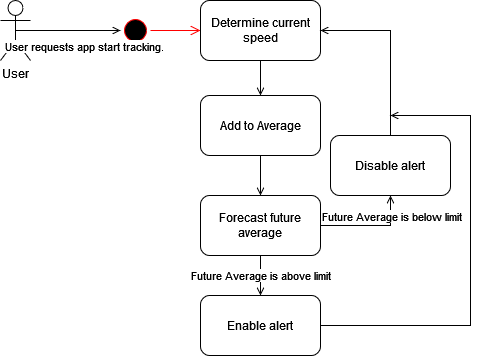
\includegraphics{UserStartedFlow.png}}
\end{figure}

The main automation is effectively a separate loop that invokes the original flow, by checking for location of the user and comparing to a dataset of average speed zones; and similarly the original flow must now return to the invocation loop when it determines it has exited a zone. This is displayed in figure \ref{fig:AutoFlow}.
\begin{figure}
    \centering
    \caption{Flow with automation.}
    \label{fig:AutoFlow}
    \scalebox{0.5}{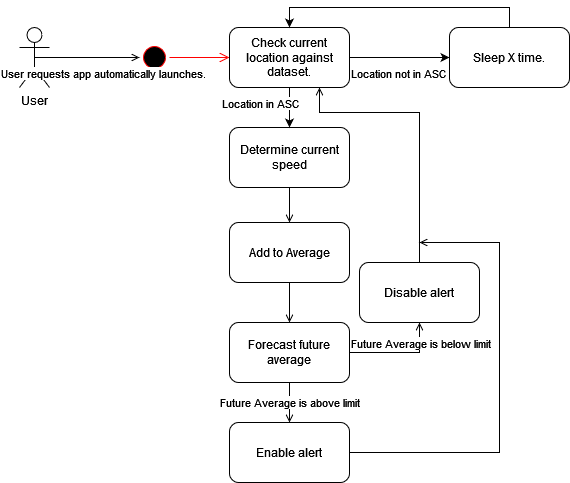
\includegraphics{AutomatedFlow.png}}
\end{figure}

\section{UI and UX Design}
A preliminary sketch of a UI was drawn on paper; this can be found in figure \ref{fig:UIPage}.
\begin{figure}
	\centering
	\caption{Preliminary UI sketch.}
	\label{fig:UIPage}
	\scalebox{1.0}{\includegraphics{UISketch.png}}
\end{figure}

\chapter{Technical Development}\label{ch:TechDev}
While the actual development of code can be found in appendix \ref{app:GitLog}, it is worthwhile discussing, separately to that, justification and reasoning behind certain decisions and implementations, as well as more general discussion about development on Android.

\section{Android Jetpack}
Android applications previously used the Android support library to allow for some form backward compatibility; Instead of the developer explicitly handling older versions, the support library allows developers to either have an implementation of "newer features on earlier versions", or "gracefully fall back to equivalent functionality" \citep{supportLibAndroid}. However since Android 9.0, the support library has been replaced by Android Jetpack libraries. Jetpack not only provides the backwards compatibility of the support libraries, but also a large amount of classes and helper functions that "help developers follow best practices, reduce boilerplate code ... so that developers can focus on the code they care about" \citep{AndroidJetpack}. Case in point with this project; the application makes use of \textit{AppCompatActivity}, which means the main activity will have a consistent appearance across previous versions of android; and the Jetpack preferences library is used as discussed below.

\section{Settings Page}
Certain parameters of the application are user configurable; for example, except for in Automatic mode, the speed limit can be changed by the user, and the forecast time for the model can be configured by the user. However, the speed limit should be changeable from the main interface of the application, while the forecast time does not need to be. Hence a "settings page" should be created.

\citet{settingsAndroid} provides a guide on how to implement a settings screen, using a \textit{PreferenceScreen} fragment. By using this part of the Android Jetpack library, a developer doesn't have to implement their own Settings system. However, to get to this settings page, the user must interact with something; one idea is for a settings button on the top bar of the application, which on Android is referred to as the "ActionBar". \citet{toolbarAndroid} provides information on how to configure an ActionBar that works across past and future android versions, and allows for action buttons. However, despite implementing this in the project, a settings button was never seen on the action bar throughout development. A future task for this project would be revisit and attempt to implement this; it is more likely to be a bug with the project's code than with the underlying Android libraries.

For testing purposes, a button to reach the settings page was explicitly added. It was removed during design of the rest of the UI, then re-added at the end. The settings page itself can be found in figure \ref{fig:settingsPage}; currently containing just two settings, but could easily be extended for further features.

\begin{figure}
	\centering
	\caption{Settings page at end of main development.}
	\label{fig:settingsPage}
	\scalebox{0.2}{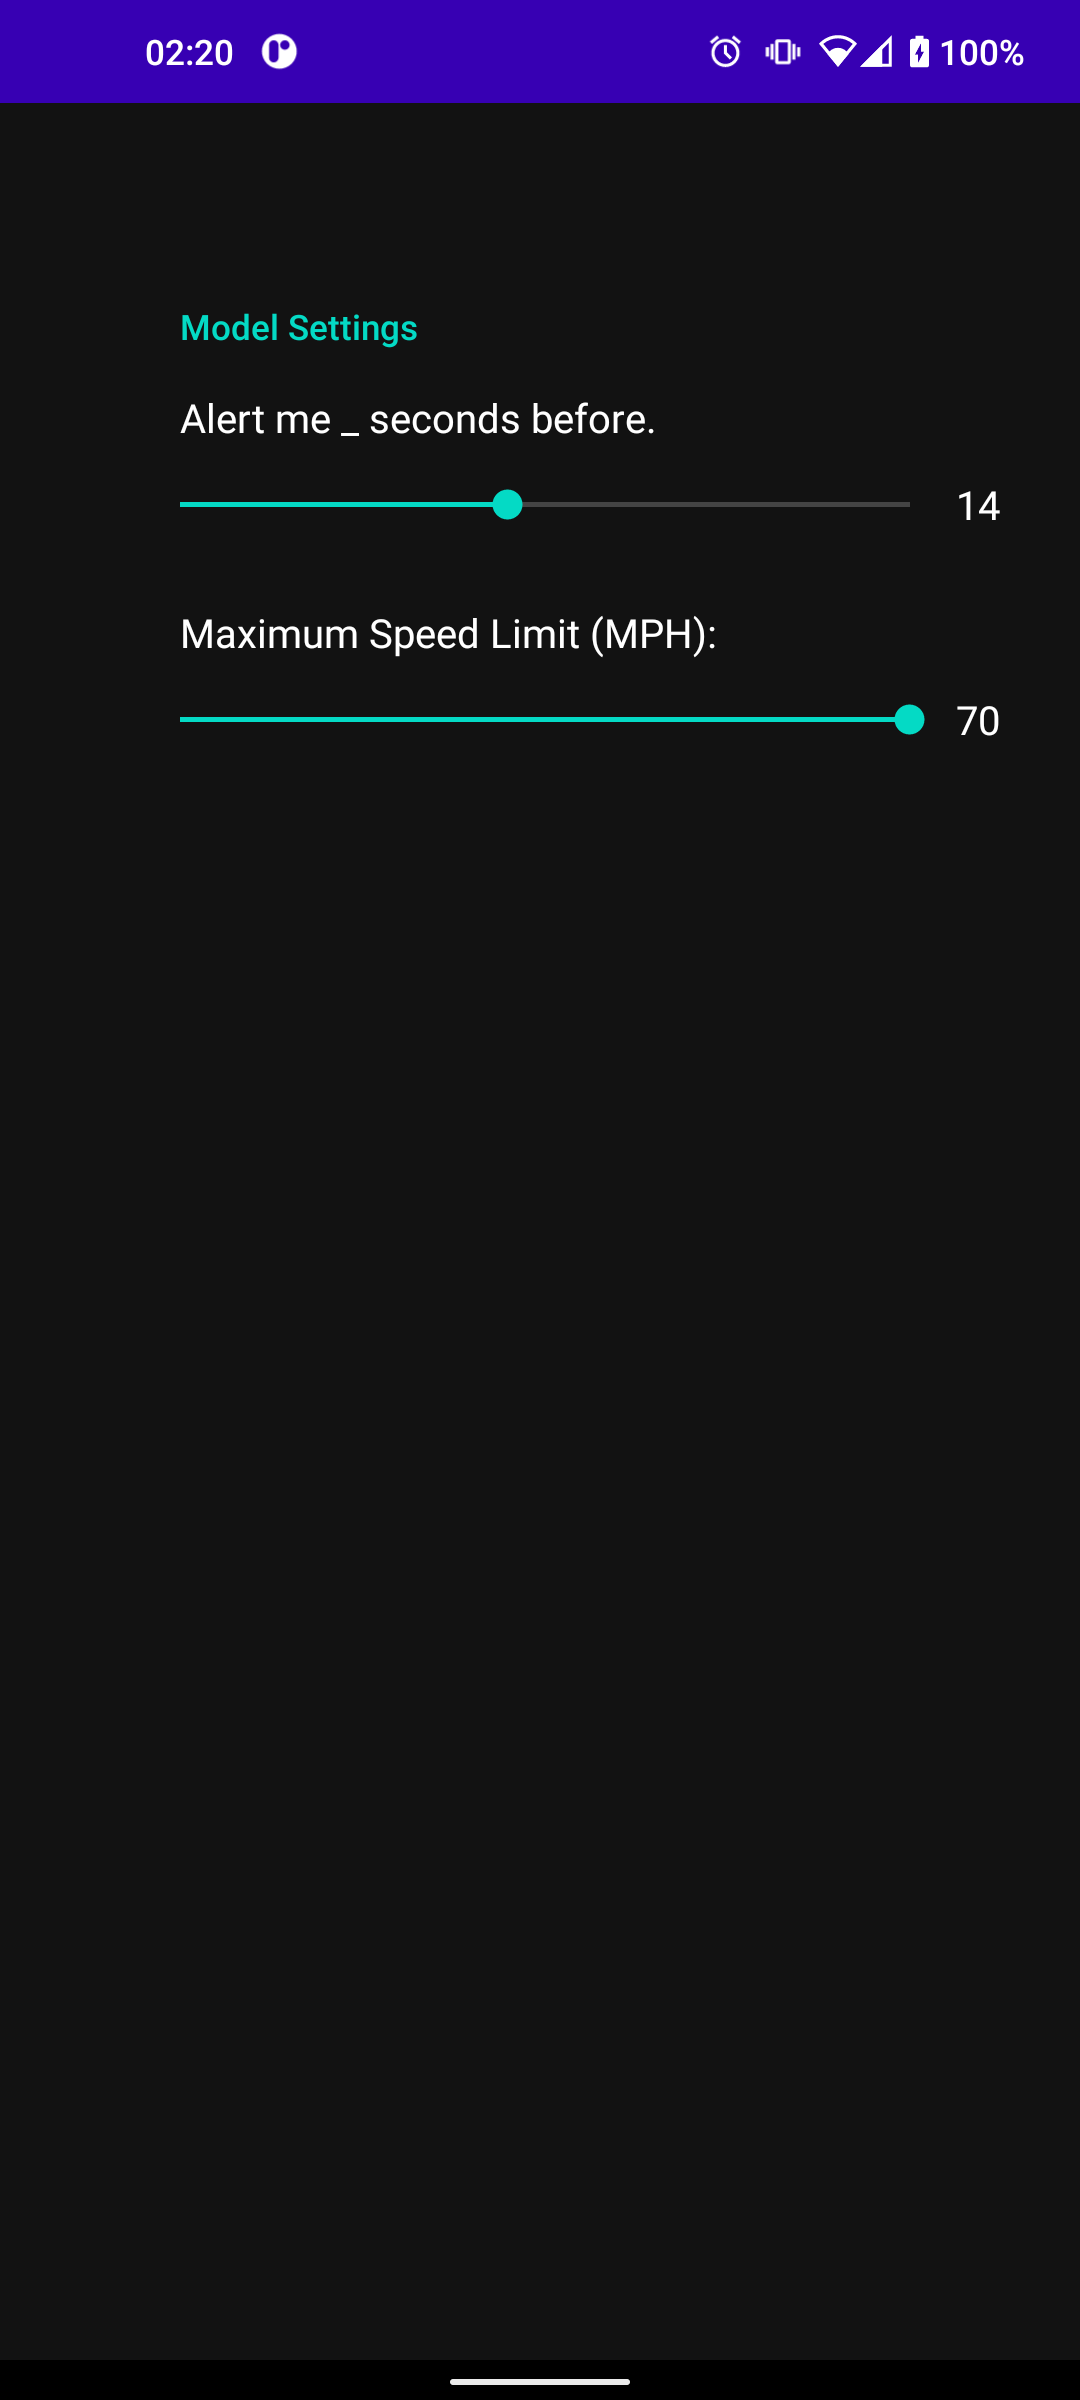
\includegraphics{SettingsPage.png}}
\end{figure}
\pagebreak

\section{Android Resources}
Android resources are "additional files and static content that your code uses" \citep{resourcesAndroid}, including images, sounds, layouts, and (static) values. In this section the use and features of some resource forms is discussed.

Resources can be "qualified" with a number of factors, such as device orientation, type, "night mode", language, etcetera; allowing for automatic reconfiguration when the device changes.

\subsection{Drawables}
Images in Android are considered to be "Drawables", and they can be either raw images in Bitmap or Vector form, or more Complex forms. For example, a file can define a StateList composed of other drawables, and code can change between them, usually based on the state of the container.

This project's only explicit use of a drawable is as a background SVG\footnote{Scalable Vector Graphics \citep{SVGW3C}} used to display the speed limit, imitating the background of a UK Speed Limit sign. However, this could become part of a StateList, with other countries backgrounds, or signs with specific meaning (E.G. the UK's National Speed Limit sign), to better improve a user's recognition of the speed limit.

The use of an SVG instead of a bitmap allows for better scaling for different UI sizes; bitmap (also known as raster) graphics are prone to artifacts on upscaling (as information has to be interpolated).

\subsection{Layouts and View Binding.}
When defining an activity's or fragment's initial state, a developer should provide a layout file that defines the initial state in XML. It is theoretically possible to build a layout in code, and it is sometimes necessary to make changes in code; when \textit{inflating} its layout, an Activity needs to add a fragment to take the place of a \textit{FragmentContainerView}. However the actual layout should be in the layout resource file, and the code should manipulate the data displayed within the layout.

Manipulating views within a layout has historically been a case of calling \textit{findViewById()} to get the view to manipulate. However this is not type safe and has few compile-time guarantees. Since Android Studio 3.6 (and the version of Jetpack released alongside it), this can be replaced by View Binding \citep{viewBindingAndroid}; upon creation of an activity or fragment, the view inflates its layout and stores the root element as a member field. Then, instead of calling findViewById(), a developer can access binding.viewId.property, which provides nullability and type-safety.

This project has a few layouts in use; two activities and two fragments, one each for the main page and the settings page. It also uses view binding in the main activity and the "DashboardFragment"; it is not necessary to do so in the settings page and fragment, as access to the components is handled preferences part of the Jetpack Library.

\subsection{Strings}
Android allows for easy localisation through the use of string resources. When the developer uses some text, the code refers to the string resource instead; based on the device's locale, this is substituted for a translated string if available.

This extraction of string resources also allows for a "single source of truth"; rather than having to find all instances of a string in code and replace them, a developer wishing to change text just has one location to alter.

Every string in the project is a string resource, but no translations have been provided.

\subsection{Integers}
Similar to the single source of truth for strings, Android resources can provide a single source of truth for Integer values. In the project this is used to set default values and limit values for the settings page.

\section{LocationManager: Getting location on Android.}
The basis of this project involves location data. Attaining objectives four, five, nine, and ten, require the use of location data; and getting speed for objectives one and two, while possible to do through other methods, is best done through the location system as explained later in this section. The first part of this is ensuring the application has the appropriate permissions; in the case of location, the application is required to request \textit{ACCESS\_FINE\_LOCATION} and \textit{ACCESS\_COARSE\_LOCATION} \citep{permissionsAndroid}. This is done in the application's manifest file, AndroidManifest.xml.

Getting location on Android involves the use of the LocationManager class \citep{locationAndroid}. LocationManager does not provide a public constructor, so code attempting to use LocationManager must get an instance in some other way. In the project, this is done through a call to \textit{context.getSystemService()} and passing in the constant \textit{Context.LOCATION\_SERVICE}; this then returns a Java \textit{Object}, so the calling code must cast the returned Object into a LocationManager.

This LocationManager instance then has two paths for a developer to get location data from it. The seemingly obvious way is to call \textit{getCurrentLocation}, which "asynchronously returns a single current location fix". However, this quickly becomes complex: this method must be called with an executor as one of the parameters, to provide which thread the callback should occur on. This in itself is not terrible to work with, but the complexity comes with calling this in a loop to constantly update the average speed; this loop should be executed on a background thread as well, so now there's a background thread managing repeated calls to another background thread, and managing the transfer of data back to the main UI thread can be difficult.

The alternative is through the use of \textit{requestLocationUpdates}. This method allows code to specify minimum distance and time between updates, and register a Listener to be executed when an update occurs. This is much easier, as the update loop and state of whether to get updates is handled by the system's LocationService and its own thread(s). When the user requests to stop tracking, this is as simple as calling \textit{removeUpdates}; this de-registers the Listener passed as a parameter (if it was already registered), and no further updates are provided.

\subsection{In the Project}
In the Project, this is implemented as the ViewModel itself being a LocationListener, and having two functions, \textit{startTracking} and \textit{stopTracking}, that call the relevant LocationManager functions. The \textit{onLocationChanged} callback function checks if the Location has a speed, and if so adds it to a mutable list, then calculates the average speed from the list.

\section{MediaPlayer: Playing sounds on Android.}
As part of objective two, the application should audibly warn the user. On Android, the default way to play an audible sound is to use an instance of MediaPlayer \citep{mediaPlayerAndroid}. Unfortunately, MediaPlayer is a very obtuse part of the Android Runtime. It works on the principle of a state machine, and this state machine is well documented and understandable; but there is no way for code interacting with it to query the state, bar a binary "isPlaying" and "isLooping" variables. The only way to handle this is for the interacting code to manually keep track of what state it "should" be in, handle callbacks, and effectively reset and start over if an error is encountered\footnote{The MediaPlayer namespace has some named errors, but most errors encountered during this project were either "attempting to pause whilst paused", or just gave back numbers with no clear meaning.}.

In this project, the class written to handle this has an internal member, \textit{isPrepared}, that keeps track of if the MediaPlayer instance is ready to play the alert sound, from the beginning. The function to start playing checks this value, and does not call play if it isn't true; if it is, then it starts playing and sets the value as false. The function to stop playing checks if this value is false and if the \textit{isPlaying} value is true, and if so pauses the player and seeks the track back to 0 seconds; a full call to the MediaPlayer's \textit{stop()} method would require going through the "prepare" flow again. Seeking is also an asynchronous operation, so during creation of the MediaPlayer, the handler registers itself for "OnSeekComplete", and it is this callback function that sets \textit{isPrepared} back to true. Through this, calls to the handler's start and stop methods are idempotent.

This is the simplest case for a handler for MediaPlayer. If this application was doing more complex things, such as playing multiple files, a more complex handler would have to be written. Regardless, it is interesting that there is no direct access to state for MediaPlayer; it suggests the internal functionality of MediaPlayer is too complex to represent the state to the user.

\section{Testing and Test-driven development.}\label{sec:TDD}
\citet{tddByExample} writes that test-driven development is when "we drive development with automated tests"; and follow the two "simple rules": "Write code only if an automated test has failed", and "eliminate duplication". A perhaps less obtuse interpretation of this, is that test-driven development is the process of writing tests first, then writing code to make those tests pass.

This project started with the intention of following the TDD methodology. However due to time constraints and management issues, all of the code was written before implementing tests; hence there is very little to talk about in terms of test result progress throughout the project. Still, there is discussion to be had about testing in general.

\subsection{Testing on Android}
\citet{testingAndroid} says "the most important distinction for app developers is where tests run"; and hence the two overall classifications for android tests: Local tests which run on the development machine, and Instrumented tests which run on an Android device, emulated or real.

Local tests are more suited for the traditional "unit tests", as when running them the overall android runtime doesn't exist, so attempting to construct Android classes (for example, LocationManager and MediaPlayer) can end up failing unless they're mocked.

In comparison, Instrumented tests are ideal for "integration tests", as they are actually run on an Android Device; meaning the android runtime exists, and test code can use android classes and contexts. In the context of the project, some instrumented tests were written in \textit{AverageSpeedModelTest.kt}; one to test that the AverageSpeedModel is instantiated to the expected state, and one to test the basic tracking functionality. However, in part due to lack of documentation around the use of LocationManager test providers, this second test fails: the AverageSpeed is reported as 0, when it should be 17. This is likely due to a delay between calls to \textit{setTestProviderLocation} and when the LocationManager actually calls the onLocationChanged callback; however, documentation on this could not be found. The solution would be manually adding a delay in the test code, but Android Instrumented tests cannot be ran in parallel on the same device, so a delay would slow down the test speed.

\section{Volley and OverpassQL: Automatically detecting ASC zones.}
Although objectives four and five were not implemented in the duration of this project, thought was given on how to do so. This section discusses their theoretical implementation.

\subsection{Public Datasets}
A brief search of \citet{OrdananceSurvey}, the \citet{ONSHome}, and data.gov.uk \citep{dataGovUK}, revealed that there were no Governmental datasets of average speed zones publicly available. Individual localities, such as \citet{sySpeedCamera}, publish the roads on which cameras are installed, but these are mostly fixed-point cameras, and they do not provide exact locations. Therefore the project would have to use a less "official" data set, or build a dataset itself (from data like South Yorkshire Safety Cameras, or field work).

\chapter{Evaluation}
This chapter evaluates the project in the context of the objectives defined in Chapter \ref{ch:AnO}, the value of the project to the public and to the author, and where the project could go in the future.

\section{Aims and Objectives.}
Due to the lack of test suite, it is hard to actually quantify whether the project meets the objectives in Chapter \ref{ch:AnO}. However in terms of what code has actually been written, only objectives one, two, and three have had code written to implement them. The lack of code for other objectives is down to aforementioned time constraints and management issues; however with respect to objectives four and five, information on how these could be achieved can be found in REFME(Refer to section - Technical Development?).

\section{Value to the Public.}
As it stands now, the project is not publicly available - hence it cannot provide any value to the public. However, should it be publicised, what code does exist can be of value to the public; it presents some basic examples of how to use view-binding, activities, fragments, and in particular a good amount of code around the use of LocationManager. As well, the application as it exists in its current state can provide some value; it does have manual tracking implemented, which could be used for the intended purpose.

\section{Value to the Author.}
During the duration of this project, the author has learnt:
\begin{itemize}
	\item About the Android development process.
	\item That said development process benefits greatly from pre-planning.
	\item About the Android development libraries, especially the the libraries discussed in Chapter \ref{ch:TechDev}.
	\item About the Kotlin programming language.
\end{itemize}
This project, then, has provided a large amount of value to the author; it has provided an opportunity to learn valuable skills, and a lesson in the utility of preparation.

\section{The Future.}
The application as it stands is close to being an MVP\footnote{Minimum Viable Product, which \citet{mvpAGuide} defines as "version of a new product which allows a team to collect the maximum amount of validated learning about customers with the least effort."}. The future of the application involves a brief refactor, then continued implementation of the objectives.

The brief refactor is required due to the use of the concrete implementation of AverageSpeedModel as opposed to an interface. Refactoring the code this way to use loose-coupling would allow for abstraction of the functionality of the model; this abstraction would then allow for the use of other models without having to refactor the code even further.

More refactoring could be done with regards to the architecture of the application. Currently there are two layers, UI and Data, but the data layer is implemented as a ViewModel, which strictly speaking is part of the UI layer \citep{UILayerAndroid}. It would be useful to redesign the architecture with the Repository pattern; the current ViewModel would mostly become a Repository, and a new ViewModel would be written.

The continued implementation of objectives involves what is discussed in REFME(Refer to section - Technical Development?) for objectives four and five. Objective six is case of implementing "App Actions" and "Built-in intents" with Google Assistant \citep{appActionsBII}, at least to allow the application to start on voice command or update the speed limit currently in use.

Objective seven would be a case of implementing a preference in the preference page, and altering the resource passed into MediaPlayer. Objective eight's implementation would be dependent on the dataset used, but in its simplest form could be a list of places stored by a voice command for the user to come back to later and add to the dataset externally; that is, the user would ask the application to remember the current location as they were entering a speed check not automatically recognised, then when finished driving, check this list against the dataset and alter it as needed.

For objectives nine and ten, this would be a case of maintaining a list of territories, and checking the current location on application start against this list. For objective eleven and twelve, a similar lookup would be required, based on the speed limit of the road when tracking is automatically started.

Bar the existing objectives, adding a choice of multiple datasets, and saving and showing previously tracked sessions are both additional features that could be implemented in the application.

\section{Conclusion.}
In conclusion: as it stands, when publicly available this project currently offers some value to the public; most of its value is as a learning experience to the author; and there is a lot possible in the future of this project.

\appendix
\chapter{Development Log}\label{app:GitLog}
Note that, as the \LaTeX\ for this report is itself hosted in the repository, this git log contains commits not relevant to the application; where possible they have been removed, but some may remain. 

% USE: git log --reverse --pretty=format:"\item %h %s %b" to get as items.
\begin{itemize}
	\item 08f4e1e Add src tree for application. 
	\item f9fbe32 Begin adding an action bar button for settings. 
	\item a254159 Remove existing action bar; attempt to add our own. Not working :(. 
	\item 4c48b0e Add button to main activity to test settings. 
	\item d44a9e4 Add SettingsPage activity. 
	\item d088240 Delete Artefacts/.idea directory Delete .idea; shouldn't be in source (technically).
	\item 1d5de89 Add SettingsFragment. 
	\item c7cbb59 Load settingsFragment in settingsPage. 
	\item f4a7c15 Change constraints on settings (still wrong but goodenough for now). 
	\item 5db6680 Implement actual setting we want. Introduce bounds and filters. 
	\item 819a055 Fix bounds and filters. 
	\item 8a456f9 Change to SeekBar. 
	\item 6d95fb5 Remove bounds, because something is wrong. 
	\item b87033e Show value on seekbar. 
	\item aecff63 Bounded seekbar. Yay. 
	\item 92b1b2c Remove uneeded filter. 
	\item cd81317 Add display fragment for average speed. 
	\item de8e5be Add background for speed limit signs. 
	\item 07eaed6 Begin adding code to model. 
	\item f79a325 Refactor averageSpeed as a property instead of function. 
	\item d467d43 Add documentation to averageSpeed. 
	\item 50780b0 Add location permissions. 
	\item f877352 Add locationConsumer. 
	\item 33115d1 Refactor to registering the model as a listener. Consider caching value instead of calculating on fly (may be a premature optimisation).
	
	Need to check for permission - pass reference into constructor just to get context?
	
	\item 1a3e899 Reimplement average speed to be calculated on update. Autogenerate permission check to implement one layer up. 
	\item ee37f3a Add speed limit to fragment\_dashboard.xml. 
	\item 7f32c1a Request location permissions on main activity creation. 
	\item 7979522 Refactor permissions check and request. Complete onRequestPermissionsResult. Move permissions to companion. 
	\item 9653c88 Fix logic error with checking results. 
	\item 94035dc Start button. 
	\item d07264f Refactor tracking to allow for stopping and starting. 
	\item d5b2906 Add documentation to MainActivity and ASModel. 
	\item 7b14d46 Enable/disable buttons. Cleanup some stuff. 
	\item 4e58df4 Toggle tracking on button. Still need to bind UI and model. 
	\item ae42405 Enable view binding in gradle. 
	\item f512479 Use view binding to replace findViewById. To actually set the average speed, I think we need to move the logic into dashboard fragment, instead of inside here.
	Equally there's going to be a pattern, involving threads no doubt, to updating the text; I imagine just setting them equal isn't going to work.
	
	\item 2c3c403 Enable binding inside of the DashboardFragment. 
	\item 6c49c4f Use binding for snackbar. 
	\item ea30396 Switch to liveData for tracking bool. 
	\item ed32d43 Use correct imports and correct onCreate. 
	\item a6d2449 Make AverageSpeedModel a ViewModel. 
	\item 68bd5b9 Observer changes to average speed and update digit text. 
	\item a955584 Add speedLimit. 
	\item 29d23c8 Observe trackingBool in DashboardFragment. 
	\item 4a546e1 Share AverageSpeedModel across fragments. 
	\item 41c46ff Access model from MainActivity. Write factory for model. 
	\item 7e93295 Add fragment-ktx dependency to allow `by activityViewModels`, etc. 
	\item 866aa14 Add AverageSpeedModelFactory and use it for initialising AverageSpeedModel. 
	\item b94bdf9 Round to int on speedo. 
	\item 0c2bfe7 Add functions to predict for model. 
	\item 34b16e1 Add and use default value in preferences. 
	\item 2527049 Pass predict time to model in startTracking. 
	\item 6acd8c3 Spelling. 
	\item 8df1b7d Add a reset to the model. 
	\item 69200f1 Predict speed and update boolean accordingly. 
	\item f1a99d9 Convert unit to mph for display. 
	\item fbdac3a Ensure no NPE with trackingBool. 
	\item aed7c9d Observe speedLimit; use non-mutable LiveData for trackingBool. Observe overSpeedLimit. 
	\item 60a0525 Need LiveData method for trackingBool. 
	\item 668d824 Move convertToUnit to static on AverageSpeedModel. 
	\item bd2d628 Extract coefficient for conversion. 
	\item b9d11c6 Get theme colour instead of black. 
	\item 8567439 Default back to white; need to work out how to get theme colour. 
	\item a711867 Tidy up. 
	\item 3b4650e Barrier comparison fix. 
	\item 75295d6 Add gesture detector to dashboard fragment. 
	\item 9b0f94e Set touch listener on Speed Limit. 
	\item 69224c9 Pad AverageSpeed. 
	\item 36e89fd We want to check the predicted speed, not if we're currently over - well, maybe not. 
	\item 879037d Set speed limit text to explicit black, since background is non-transparent white. 
	\item cf891d1 Add bounds checks on speed limit. 
	\item 96feeec I promise 350 was a test value. Upper bound is 70 since UK roads have no higher limit. 
	\item 91a7099 Allow setting maximum speed limit in settings; extract prefMan as a member to reduce redundancy. 
	\item 813ae34 Merge remote-tracking branch 'origin/allowSetSpeedLimit' 
	\item c4a7cd6 Change default invocation of model to use speed limit of 30. 
	\item 44c661e Add overLimit.ogg, which is from https://notificationsounds.com/message-tones/maybe-552; need to attribute (CC-BY-4.0-IL). 
	\item a2dd992 Rename resource; begin adding code ot asynchronously get mediaPlayer. 
	\item 78e4df0 Extract function; null mediaPlayer after release. 
	\item 584e01a Set night colonOnSecondary to white. 
	\item b1397e1 Get onSecondary from theme. 
	\item 58cc052 Move to URI Builder to not have issues. 
	\item 2d16ea5 Merge branch 'fixStaticColor' 
	\item a186183 Handle proper destruction of mediaPlayer. 
	\item 3445da4 Add inner class to handle media player events. 
	\item c3abfbd Proper param names; actual error handling. 
	\item ff1bb96 Actually use handler methods to start/stop limit sound. 
	\item 15e5322 Handle case where we already have mediaPlayer. 
	\item 9884fba Say we didn't handle this error if it's not our mediaPlayer. 
	\item 6f13d01 Handle synchronous exceptions. 
	\item e2bb493 Begin writing testing for AverageSpeedModel. 
	\item 359c3b6 Set default speedLimit to 30 MPH. 
	\item 6ce69f8 Add test to test setting up test functions. 
	\item 2f2694a Disable minify on debug build. 
	\item 3bdab20 Switch to instrumented test. 
	\item 6913481 Enable Jetifier. 
	\item 84eabbc Explicitly add androidx Core and androidx.test dependencies. 
	\item 331cbed Working Instrumented Test! 
	\item e367c9c Suppress warning; we manually gave permission for testing. 
	\item bddd100 Add more tests. 
	\item cbd414f Fix issues with times and accuracy; invert asserts to proper direction; add assert at end of checkBasicTracking. 
	\item 2d56328 Re-add explicit button for settings.
\end{itemize}

\bibliography{finalrep}
\end{document}